
\begin{problem}[Question:]{Longest Increasing Subarray | Kadan's Algorithm}
    You are given a array of number, find the longest \textbf{subarray} whose sum is maximum.
\end{problem}

\begin{solution}[Naive]
    \rfl{For all subarray problem, please note that iterative solution is the most natural choise.}
    This is same as for all \underline{subsequence} and \underline{subsequence count problem},recursion is the most natural choice.

    \medskip
    \intution{Let $dp[idx,\_]$ be the the maximum subarray sum, that ends at idx \& \textbf{contains idx}.
    Lets try to write up dp[idx] in terms of subproblem.}
    \footnote{i.e assume that we already know the subproblem answer, now just express dp[idx] in terms of subproblems.}
    
    \medskip
    At dp[idx], we have two choices:
    \begin{asparaenum}[(a)]
        \item \indent Continue the previous subarray. $(val_1 = dp[idx-1]+arr[idx])$
        \item Start a new subarray. $(val_2 = arr[idx])$
    \end{asparaenum}

    \begin{marginfigure}
        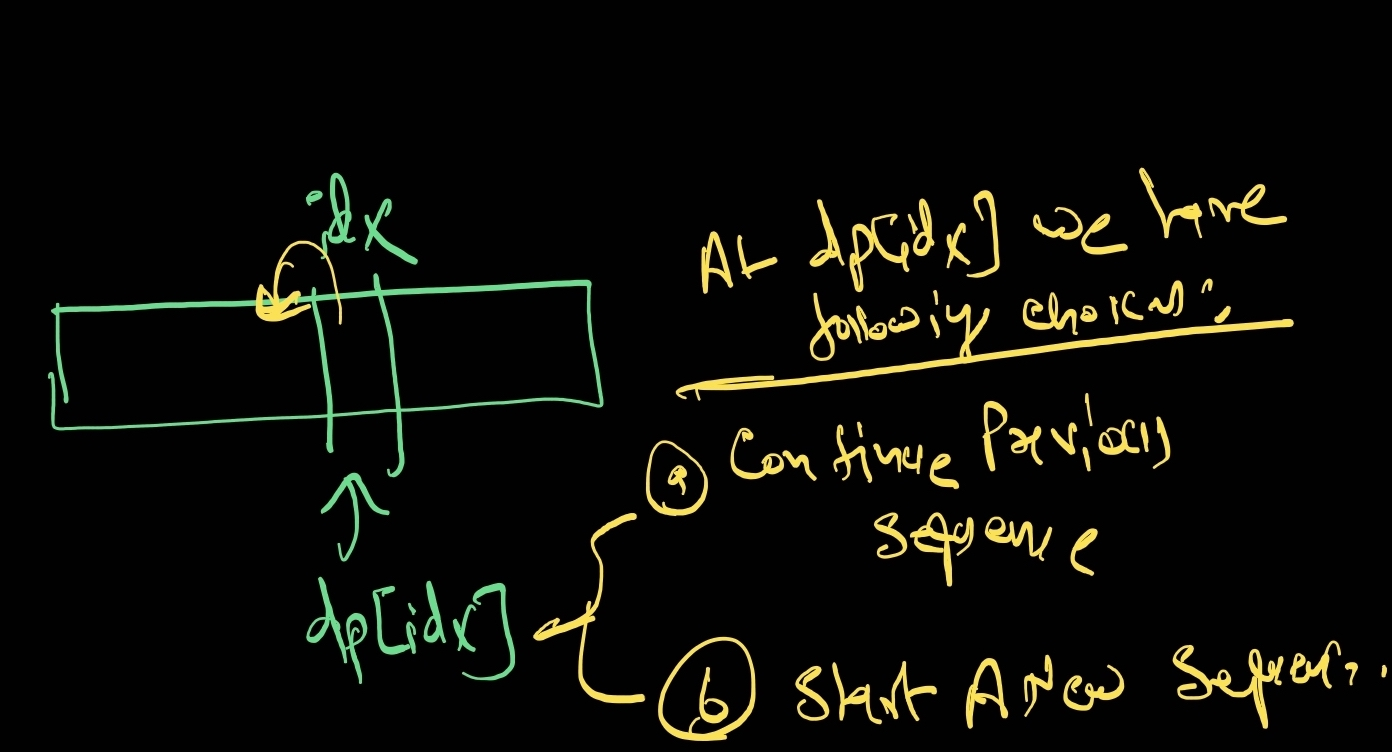
\includegraphics[width=\marginparwidth]{./resources/KadansChoices.jpg}
    \end{marginfigure}

    \medskip
    Hence, for idx we take the best of both $dp[idx] = max(val_1,val_2)$. \\[2mm]
    Now,as we got the maximum subarray when the arr[idx] must be included in the end point of subarray. Our answer be the the maximum amoung all dp[idx].


    \begin{figure}
    \begin{verbatim}
        int maxSubArray(vector<int>& arr) 
        {
            
            int size = arr.size();
            vector<int> dp(arr);
            
            for(int idx=1;idx<size;idx++)
            {
                dp[idx] = max(arr[idx]+dp[idx-1], arr[idx]);
            }

            return *max_element(dp.begin(),dp.end());
    
        }
    \end{verbatim}
\end{figure}

\end{solution}